
\documentclass[12pt,a4paper]{article}

% ── Packages ──────────────────────────────────────────────────────────────────
\usepackage[utf8]{inputenc}
\usepackage[T1]{fontenc}
\usepackage{lmodern}
\usepackage[margin=1in]{geometry}
\usepackage{amsmath, amssymb, amsthm}
\usepackage{bm}
\usepackage{booktabs}
\usepackage{array}
\usepackage{tabularx}
\usepackage{graphicx}
\usepackage{float}
\usepackage{caption}
\usepackage{subcaption}
\usepackage{xcolor}
\usepackage{hyperref}
\usepackage{algorithm}
\usepackage{algpseudocode}
\usepackage{natbib}
\usepackage{doi}
\usepackage{setspace}
\usepackage{parskip}
\usepackage{microtype}
\usepackage{enumitem}
\usepackage{titlesec}
\usepackage{csvsimple}
\usepackage{siunitx}

% ── Hyperref setup ─────────────────────────────────────────────────────────────
\hypersetup{
    colorlinks=true,
    linkcolor=blue!60!black,
    citecolor=green!50!black,
    urlcolor=cyan!60!black,
    pdftitle={Dynamic Soft-Thresholding via Iteratively Reweighted Proximal Gradient for Feature Selection in High-Dimensional Regression},
    pdfauthor={Yash Karecha; Tenzin Kunga}
}

% ── Math operators ─────────────────────────────────────────────────────────────
\DeclareMathOperator{\sign}{sign}
\DeclareMathOperator{\prox}{prox}
\newcommand{\R}{\mathbb{R}}
\newcommand{\norm}[1]{\left\|#1\right\|}
\newcommand{\abs}[1]{\left|#1\right|}
\newcommand{\csvtablepath}[1]{\IfFileExists{outputs/tables/#1}{outputs/tables/#1}{../outputs/tables/#1}}
\graphicspath{{outputs/figures/}{../outputs/figures/}}

% Compact numeric rendering to avoid table overflow.
\newcommand{\fmtpred}[1]{\num[round-mode=places,round-precision=2,group-separator={}]{#1}}
\newcommand{\fmtjac}[1]{\num[round-mode=places,round-precision=4,group-separator={}]{#1}}



% ── Theorem environments ───────────────────────────────────────────────────────
\newtheorem{remark}{Remark}

% ── Line spacing ───────────────────────────────────────────────────────────────
\onehalfspacing

% ══════════════════════════════════════════════════════════════════════════════
\begin{document}

% ── Title block ───────────────────────────────────────────────────────────────
\begin{titlepage}
    \centering
    \vspace*{2cm}
    {\LARGE\bfseries Dynamic Soft-Thresholding via Iteratively Reweighted\\[0.4em]
    Proximal Gradient for Feature Selection in\\[0.4em]
    High-Dimensional Regression\par}
    \vspace{1.5cm}
    {\large Yash Karecha and Tenzin Kunga\par}
    \vspace{0.3cm}
    {\normalsize B.Tech, Computer Science (AI/ML), 3rd Year\par}
    \vspace{0.5cm}
    {\normalsize Numerical Optimisation --- Theme 3 Project\par}
    \vspace{0.5cm}
    {\normalsize \today\par}
\end{titlepage}

\begin{abstract}
    \noindent
    High-dimensional tabular regression often involves many correlated predictors,
    only a subset of which contributes meaningful signal.  While LASSO promotes
    sparsity, it can be unstable under multicollinearity and may over-shrink large
    coefficients; Elastic Net \citep{zouhastie2005} improves grouping behaviour but
    does not necessarily yield sparser models.  We implement and evaluate
    \textbf{IRL1-PG}, combining Iteratively Reweighted $\ell_1$ Minimisation
    \citep{candes2008} with ISTA/FISTA proximal gradient solvers \citep{beck2009}.
    On the Kaggle \emph{House Prices: Advanced Regression Techniques} benchmark, we
    compare dynamic IRL1-PG against Ridge, standard LASSO, and static Adaptive LASSO
    \citep{zou2006} under matched preprocessing and data splits.  The best dynamic
    settings reach validation MSE $7.79\times 10^8$ (ISTA) and test MSE
    $8.29\times 10^8$ (FISTA), outperforming Ridge and LASSO while using only 92--99
    non-zero coefficients versus 240--283 in baseline models.  FISTA, motivated by
    Nesterov acceleration \citep{nesterov1983}, improves test MAE over ISTA at nearly
    identical runtime.  We do not claim algorithmic novelty; the contribution is a
    careful and reproducible empirical analysis of IRL1-PG in a correlated tabular
    regression setting.
\end{abstract}

\newpage

\tableofcontents
\newpage

% ══════════════════════════════════════════════════════════════════════════════
\section{Introduction}
\label{sec:intro}

High-dimensional regression is often challenging in practice, especially when the number
of features is much larger than the number of observations.  In domains such as real
estate pricing, gene expression studies, and finance, datasets often contain hundreds
of predictors, but many of them are either redundant or weakly informative.  If all
features are used without control, models tend to overfit, generalise poorly, and lose
interpretability.  This motivates sparse modelling: retaining only the coefficients
that carry meaningful predictive signal.

LASSO (Least Absolute Shrinkage and Selection Operator), introduced by
\citet{tibshirani1996}, became popular because adding an $\ell_1$ penalty to least
squares drives many coefficients exactly to zero.  However, LASSO is not without
limitations.  With highly correlated predictors, it can behave unstably: selecting one
variable from a correlated group arbitrarily, over-shrinking important coefficients,
or missing relevant predictors depending on the design structure
\citep{huang2008}.

To address correlation effects, \citet{zouhastie2005} proposed the Elastic Net, which
combines $\ell_1$ and $\ell_2$ penalties so correlated variables are more likely to be
selected or removed together.  This improves grouping behaviour, but Elastic Net does
not typically produce greater sparsity than LASSO, so it is not the main focus here.

Adaptive LASSO, proposed by \citet{zou2006}, extends this idea by assigning
feature-specific penalty weights obtained from an initial estimator (for example Ridge
or least squares).  With appropriately chosen weights, Adaptive LASSO can recover the
correct support and achieve asymptotically efficient estimation, commonly described as
having \textbf{oracle properties} \citep{huang2008}.

A broader framework is \textbf{Iteratively Reweighted $\ell_1$ Minimisation (IRL1)},
introduced by \citet{candes2008}.  Instead of fixing weights once, IRL1 updates the
weights at each outer iteration based on the current coefficient estimates.  A related
family, Iteratively Reweighted Least Squares (IRLS), solves reweighted $\ell_2$
sub-problems with the same goal of approximating the ideal sparse $\ell_0$ objective
\citep{daubechies2009}.  \citet{wipf2011} showed that IRL1 and IRLS can be viewed as
alternative procedures for minimising concave surrogate penalties of $\ell_0$.

In our project, IRL1 is integrated into a proximal gradient solver, yielding the
\textbf{IRL1-PG} algorithm.  The implementation supports both ISTA and accelerated
FISTA; the latter follows Nesterov's momentum framework \citep{nesterov1983}, which
achieves faster convergence for smooth convex problems.  We evaluate IRL1-PG on the
House Prices: Advanced Regression Techniques dataset and compare it against Ridge,
standard LASSO, and static Adaptive LASSO (with fixed weights).  The objective is not
to claim algorithmic novelty, but to provide a careful empirical analysis of how
IRL1-PG behaves in correlated, real-world tabular regression settings.

% ══════════════════════════════════════════════════════════════════════════════
\section{Related Work}
\label{sec:related}

\subsection{LASSO and Proximal Gradient Methods}

LASSO was introduced by \citet{tibshirani1996} and tackles the objective
\begin{equation}
    \min_{\beta} \; \frac{1}{2n}\norm{y - X\beta}_2^2 + \lambda \norm{\beta}_1.
    \label{eq:lasso}
\end{equation}
The $\ell_1$ penalty is convex but non-smooth, which makes standard gradient descent
problematic at points where coefficients hit zero.  For this composite setting,
the standard optimisation framework is \textbf{proximal gradient descent}
\citep{parikh2014}.  If the objective is split as $f(\beta) + g(\beta)$, where
$f$ is smooth and $g$ is convex but non-smooth, the update is
\begin{equation}
    \beta^{k+1} = \prox_{\alpha g}\!\left(\beta^k - \alpha \nabla f(\beta^k)\right),
    \label{eq:proxgrad}
\end{equation}
where $\alpha > 0$ is the step size and $\prox_{\alpha g}$ is the proximal operator.
When $g(\beta) = \lambda\norm{\beta}_1$, this becomes coordinate-wise soft-thresholding
\citep{beck2009}.  The method converges at rate $O(1/k)$ provided that
$\alpha \leq 1/L$, where $L$ is the Lipschitz constant of $\nabla f$.

\subsection{Elastic Net}

Elastic Net, proposed by \citet{zouhastie2005}, blends LASSO and ridge penalties:
\begin{equation}
    \min_{\beta} \; \frac{1}{2n}\norm{y - X\beta}_2^2
    + \lambda_1 \norm{\beta}_1 + \lambda_2 \norm{\beta}_2^2.
    \label{eq:elasticnet}
\end{equation}
Its key property is the \emph{grouping effect}: highly correlated predictors tend to
enter or leave the model together.  This is particularly useful when predictors
outnumber samples.  Even so, Elastic Net typically does not deliver the additional
sparsity observed with iterative reweighting, so in this work it serves as a useful
baseline rather than a direct alternative to IRL1-PG.

\subsection{FISTA---Accelerated Proximal Gradient}

\citet{beck2009} extended ISTA with a Nesterov-style momentum term to obtain FISTA,
achieving faster convergence without increasing per-iteration complexity.  Grounded in
Nesterov's \citeyearpar{nesterov1983} acceleration framework for smooth convex
objectives, FISTA reaches a convergence rate of $O(1/k^2)$.  The momentum sequence is
initialised with $t_1 = 1$ and updated by
\begin{equation}
    t_{k+1} = \frac{1 + \sqrt{1 + 4t_k^2}}{2},
    \label{eq:fista_t}
\end{equation}
with an extrapolation step applied before each proximal update.

\subsection{Adaptive LASSO and Oracle Properties}

\citet{zou2006} proposed Adaptive LASSO, which introduces feature-specific weights:
\begin{equation}
    \min_{\beta} \; \frac{1}{2n}\norm{y - X\beta}_2^2
    + \lambda \sum_{j=1}^{p} w_j \abs{\beta_j},
    \label{eq:adalasso}
\end{equation}
where $w_j = 1/\abs{\hat{\beta}_j^{\mathrm{init}}}^\gamma$.  \citet{huang2008} extended
oracle analysis to the high-dimensional $p > n$ regime, showing that consistent
variable selection remains possible under partial orthogonality assumptions.  The main
limitation in practice is that static Adaptive LASSO fixes these weights after the
initial estimate and does not adapt them during optimisation.

\subsection{Iteratively Reweighted $\ell_1$ and $\ell_2$ Methods}

\citet{candes2008} introduced IRL1 as a way to approximate the $\ell_0$ objective more
closely than standard $\ell_1$ minimisation by solving a sequence of weighted $\ell_1$
problems:
\begin{equation}
    \beta^{(k+1)} = \arg\min_\beta \; \frac{1}{2n}\norm{y - X\beta}_2^2
    + \lambda \sum_{j=1}^{p} w_j^{(k)} \abs{\beta_j}, \quad
    w_j^{(k)} = \frac{1}{\left(\abs{\beta_j^{(k)}} + \epsilon\right)^\gamma}.
    \label{eq:irl1_outer}
\end{equation}
This weighting rule approximates the log-sum penalty
$\sum_j \log(\abs{\beta_j} + \epsilon)$, which is a concave surrogate for the
$\ell_0$ norm.  In parallel, IRLS \citep{daubechies2009} uses reweighted
$\ell_2$ sub-problems to target the same sparse-recovery objective, with convergence
results under restricted isometry conditions.  \citet{wipf2011} unify these views,
showing that both reweighted $\ell_1$ and $\ell_2$ methods can be interpreted as
optimising concave, sparsity-inducing merit functions.

% ══════════════════════════════════════════════════════════════════════════════
\section{Methodology}
\label{sec:method}

\subsection{Problem Setup}

Let $X \in \R^{n \times p}$ be the standardised design matrix, $y \in \R^n$ the
response vector, and $\beta \in \R^p$ the coefficient vector.  We write the smooth
loss term as
\begin{equation}
    f(\beta) = \frac{1}{2n}\norm{y - X\beta}_2^2,
    \label{eq:smooth}
\end{equation}
with gradient
\begin{equation}
    \nabla f(\beta) = -\frac{1}{n}X^\top(y - X\beta).
    \label{eq:gradient}
\end{equation}
For this quadratic loss, $\nabla f$ is Lipschitz continuous with constant
\begin{equation}
    L = \frac{\lambda_{\max}(X^\top X)}{n},
    \label{eq:lipschitz}
\end{equation}
so any step size $\alpha \in (0, 1/L]$ is valid \citep{parikh2014}.

\subsection{Weighted Proximal Operator and Soft-Thresholding}

For the weighted $\ell_1$ penalty $g(\beta) = \lambda \sum_j w_j \abs{\beta_j}$ with
weight vector $w \in \R^p_{>0}$, the proximal operator is separable and admits a
closed-form solution.  For a gradient step $z = \beta - \alpha \nabla f(\beta)$, the
proximal update is coordinate-wise \textbf{weighted soft-thresholding}:
\begin{equation}
    \beta_j^{+} = \sign(z_j)\max\!\left(\abs{z_j} - \alpha \lambda w_j,\; 0\right).
    \label{eq:wst}
\end{equation}
Each coordinate survives only when $\abs{z_j}$ exceeds the
coordinate-specific threshold $\tau_j = \alpha \lambda w_j$.

\begin{remark}[Connection to $\ell_1$ subdifferential]
The subdifferential of $\abs{\beta_j}$ is
\begin{equation}
    \partial \abs{\beta_j} =
    \begin{cases}
        \{\sign(\beta_j)\} & \beta_j \neq 0 \\
        [-1,\, 1]           & \beta_j = 0.
    \end{cases}
    \label{eq:subdiff}
\end{equation}
The IRL1 weight $w_j^{(k)}$ acts as a continuous indicator of how close a coordinate
is to the non-differentiable point at zero.  Large $\abs{\beta_j}$ leads to a smaller
weight and a weaker threshold; small $\abs{\beta_j}$ leads to a larger weight and
stronger shrinkage toward zero \citep{candes2008}.
\end{remark}

\subsection{Initialisation and the Pruning Mechanism}

At initialisation $\beta^{(0)} = \mathbf{0}$, all weights equal
$w_j^{(0)} = 1/\epsilon^\gamma$---the maximum possible value.  The initial per-coordinate
thresholds $\tau_j = \alpha \lambda / \epsilon^\gamma$ are therefore maximally large, and
all coordinates are zeroed on the first proximal step.  As optimisation proceeds, features
that carry genuine signal grow in magnitude, causing their weights to decrease and
thresholds to relax.  Irrelevant features remain near zero, sustain high weights, and are
repeatedly zeroed.  This progressive refinement of a small active set follows directly
from the IRL1 weight schedule \citep{wipf2011}, rather than a separate manual rule.

\subsection{IRL1 Weight Update}

After each outer iteration the weights are recomputed as \citep{candes2008}:
\begin{equation}
    w_j^{(k)} = \frac{1}{\left(\abs{\beta_j^{(k)}} + \epsilon\right)^\gamma},
    \label{eq:irl1_weights}
\end{equation}
where $\gamma > 0$ controls how aggressively small coefficients are penalised, and
$\epsilon > 0$ ensures numerical stability near zero.

\subsection{ISTA Inner Solver}

For fixed weights $w^{(k)}$, the weighted LASSO sub-problem is solved using ISTA
\citep{beck2009}.  At inner iteration $t$:
\begin{enumerate}[noitemsep]
    \item Compute gradient: $g = \nabla f(\beta^t) = -\frac{1}{n}X^\top(y - X\beta^t)$
    \item Gradient step: $z = \beta^t - \alpha g$
    \item Proximal step: $\beta^{t+1}_j = \sign(z_j)\max(\abs{z_j} - \alpha\lambda w_j^{(k)},\, 0)$
\end{enumerate}
With fixed weights and $\alpha \leq 1/L$, ISTA converges at rate $O(1/t)$ for this
convex sub-problem.

\subsection{FISTA Inner Solver}

FISTA replaces the ISTA update with a momentum-accelerated variant \citep{beck2009},
rooted in Nesterov's \citeyearpar{nesterov1983} accelerated gradient framework.
Initialise $t_1 = 1$, $y^1 = \beta^0$.  At inner iteration $t$:
\begin{enumerate}[noitemsep]
    \item Proximal step from momentum point:
          $\beta^{t+1}_j = \sign(y^t_j - \alpha g_j) \cdot \max(\abs{y^t_j - \alpha g_j}
          - \alpha\lambda w_j^{(k)},\, 0)$
    \item Update momentum coefficient:
          $t_{t+1} = \frac{1 + \sqrt{1 + 4t_t^2}}{2}$
    \item Momentum point for next step:
          $y^{t+1} = \beta^{t+1} + \frac{t_t - 1}{t_{t+1}}(\beta^{t+1} - \beta^t)$
\end{enumerate}
For the fixed-weight sub-problem, FISTA achieves $O(1/t^2)$ convergence, improving on
ISTA without increasing per-iteration complexity.

\subsection{Stopping Criterion}

The inner solver terminates when the relative change in the coefficient vector falls
below tolerance:
\begin{equation}
    \frac{\norm{\beta^{\mathrm{curr}} - \beta^{\mathrm{prev}}}_2}
         {\max\!\left(1,\; \norm{\beta^{\mathrm{prev}}}_2\right)} < \mathrm{tol}.
    \label{eq:stopping}
\end{equation}
The denominator $\max(1, \norm{\beta^{\mathrm{prev}}}_2)$ avoids spurious early
stopping when coefficients are still close to zero \citep{parikh2014}.

\subsection{IRL1-PG: Full Algorithm}

\begin{algorithm}[H]
\caption{IRL1-PG (Iteratively Reweighted $\ell_1$ Proximal Gradient)}
\label{alg:irl1pg}
\begin{algorithmic}[1]
\Require $X,\, y,\, \lambda,\, \gamma,\, \epsilon,\, \alpha,\,
          \texttt{max\_outer},\, \texttt{max\_inner},\, \texttt{tol}$
\State $\beta \leftarrow \mathbf{0}$,\quad
       $w_j \leftarrow 1/\epsilon^\gamma \;\forall j$
\For{$k = 1$ \textbf{to} \texttt{max\_outer}}
    \State $\beta_{\mathrm{prev}} \leftarrow \beta$
    \State $\beta \leftarrow \textsc{ISTA-or-FISTA}(X,\, y,\, \lambda,\, w,\, \alpha,\,
           \texttt{max\_inner},\, \texttt{tol})$
    \State $w_j \leftarrow 1 / (\abs{\beta_j} + \epsilon)^\gamma \;\forall j$
    \State $w \leftarrow \mathrm{clip}(w,\, w_{\max})$
    \If{$\norm{\beta - \beta_{\mathrm{prev}}}_2 / \max(1, \norm{\beta_{\mathrm{prev}}}_2)
        < \texttt{tol\_outer}$}
        \State \textbf{break}
    \EndIf
\EndFor
\State \Return $\beta$
\end{algorithmic}
\end{algorithm}

\subsection{Convergence Scope}

\begin{remark}[Scope of convergence guarantees]
Because $w^{(k)}$ changes at every outer step, the objective itself changes across
outer iterations.  Classical ISTA/FISTA guarantees---stated for a \emph{fixed}
objective \citep{beck2009}---therefore apply to each inner solve, but not directly to
the full outer sequence $\{\beta^{(k)}\}$.  Existing IRL1 analyses
\citep{candes2008,wipf2011} support convergence to local minima of concave
approximations such as the log-sum penalty under mild assumptions.  In this work, we
evaluate outer-loop behaviour empirically using objective traces, coefficient changes,
and sparsity trajectories across iterations.
\end{remark}

% ══════════════════════════════════════════════════════════════════════════════
\section{Experimental Setup}
\label{sec:experiments}

\subsection{Dataset}

The \textbf{House Prices: Advanced Regression Techniques} dataset \citep{kaggle2019} is a
tabular regression benchmark with 1,460 training observations and 79 raw features
describing residential properties in Ames, Iowa.  The prediction target is the raw sale
price (\texttt{SalePrice}) without log transformation.  After one-hot encoding categorical
features, the design matrix typically contains 200--250 columns, making it a suitable
high-dimensional regression benchmark with strong multicollinearity---for example, between
\texttt{GrLivArea}, \texttt{1stFlrSF}, and \texttt{TotalBsmtSF}, and among the various
quality score indicators.  This setting is precisely the type where standard LASSO
exhibits instability \citep{zouhastie2005} and where reweighted methods are expected to
improve upon it \citep{candes2008}.

\subsection{Preprocessing Protocol}

\begin{enumerate}[noitemsep]
    \item \textbf{Missing values:} Numeric features imputed with column median;
            categorical features imputed with the most frequent category from the
            training split.
    \item \textbf{Encoding:} One-hot encoding for all categorical features; original
          category columns dropped.
    \item \textbf{Scaling:} All numeric features standardised to zero mean and unit
            variance after splitting, using parameters estimated on the training set only
            (to avoid leakage).
    \item \textbf{Target:} Raw \texttt{SalePrice} (no log transformation).
    \item \textbf{Split:} 70\% train / 10\% validation / 20\% test, using a random split
          with a fixed seed and no stratification.
\end{enumerate}

\subsection{Methods Compared}

\begin{table}[H]
\centering
\caption{Summary of methods compared in the experiment.}
\label{tab:methods}
\begin{tabularx}{\textwidth}{llllX}
\toprule
\textbf{Method} & \textbf{Type} & \textbf{Solver} & \textbf{Weights} \\
\midrule
Ridge                      & Baseline & \texttt{sklearn.RidgeCV}  & N/A \\
Standard LASSO             & Baseline & \texttt{sklearn.LassoCV}  & Uniform ($w_j = 1$) \\
Static Adaptive LASSO      & Baseline & Custom ISTA/FISTA         & Fixed from Ridge init \\
IRL1-PG + ISTA             & Proposed & Custom ISTA               & Updated per outer iter \\
IRL1-PG + FISTA            & Proposed & Custom FISTA              & Updated per outer iter \\
\bottomrule
\end{tabularx}
\end{table}

\noindent\textbf{Note:} The accuracy comparison (MSE, MAE) includes sklearn baselines
because they provide reliable reference performance from standard implementations.  The
optimiser-efficiency comparison (iterations, runtime) is restricted to custom
ISTA/FISTA variants only, so solver behaviour is compared under matched stopping rules.

\subsection{Hyperparameter Search}

Grid search over the validation set:
\begin{itemize}[noitemsep]
    \item $\lambda \in [10^{-4},\; 1.0]$ (15 values, log-spaced)
    \item $\gamma \in \{0.5,\; 1.0,\; 2.0\}$
    \item $\epsilon \in \{10^{-3},\; 10^{-4}\}$
    \item \texttt{max\_outer\_iter} $\in \{5,\; 10,\; 20\}$
\end{itemize}
Step size: $\alpha = 0.99/L$ where $L = \lambda_{\max}(X^\top X)/n$, computed once from
the training matrix.

\subsection{Evaluation Metrics}

\begin{itemize}[noitemsep]
    \item \textbf{Predictive accuracy:} MSE and MAE on validation and test sets.
    \item \textbf{Sparsity:} $\norm{\hat{\beta}}_0$ (number of non-zero coefficients
          after thresholding at $10^{-6}$).
    \item \textbf{Feature selection stability:} Jaccard index
          $J(A,B) = \abs{A \cap B}\,/\,\abs{A \cup B}$ of selected feature sets across
          5 random seeds.
    \item \textbf{Optimiser efficiency:} Wall-clock runtime (seconds) and number of total
          inner iterations to convergence, for custom solvers only.
\end{itemize}

% ══════════════════════════════════════════════════════════════════════════════
\section{Results and Discussion}
\label{sec:results}

\subsection{Predictive Performance}

\begin{table}[H]
\centering
\caption{Predictive performance and sparsity loaded from \texttt{full\_comparison\_table.csv}.}
\label{tab:results}
\scriptsize
\begin{tabular}{llrrrr}
\toprule
\textbf{Method} & \textbf{Val MSE} & \textbf{Test MSE} & \textbf{Test MAE} & \textbf{Non-zeros} & \textbf{Runtime (s)}\\
\midrule
Ridge & \fmtpred{787378459.1835155} & \fmtpred{865125926.2297935} & \fmtpred{18647.05160813634} & 283 & \fmtpred{0.0240332759994998}\\
LASSO & \fmtpred{895357083.9040277} & \fmtpred{894021355.3213253} & \fmtpred{19470.818271987737} & 240 & \fmtpred{3.26278962699962}\\
Adaptive LASSO & \fmtpred{911144802.0004896} & \fmtpred{894529896.3746411} & \fmtpred{19505.95387464254} & 282 & \fmtpred{0.0855895559998316}\\
Dynamic IRL1-ISTA & \fmtpred{778965140.9490047} & \fmtpred{830975941.2048745} & \fmtpred{18186.17699240722} & 99 & \fmtpred{0.2207678519989713}\\
Dynamic IRL1-FISTA & \fmtpred{798430563.0702212} & \fmtpred{828667214.9136565} & \fmtpred{17935.6266319796} & 92 & \fmtpred{0.23186815900135116}\\
\bottomrule
\end{tabular}
\end{table}

Key observations are as follows:
\begin{itemize}[noitemsep]
    \item On this split, dynamic IRL1-PG outperforms static Adaptive LASSO in both predictive error and sparsity.
    \item Relative to Ridge, IRL1-PG (FISTA) improves test MSE by approximately $4.21\%$
        and reduces selected features from 283 to 92.
    \item Relative to standard LASSO, IRL1-PG (FISTA) improves test MSE by approximately $7.31\%$
        and test MAE by approximately $7.88\%$, while selecting fewer features.
    \item Within dynamic variants, ISTA attains lower validation MSE, while FISTA achieves the
        best test MSE and test MAE.
\end{itemize}

\subsection{Convergence Analysis}

\begin{figure}[H]
    \centering
    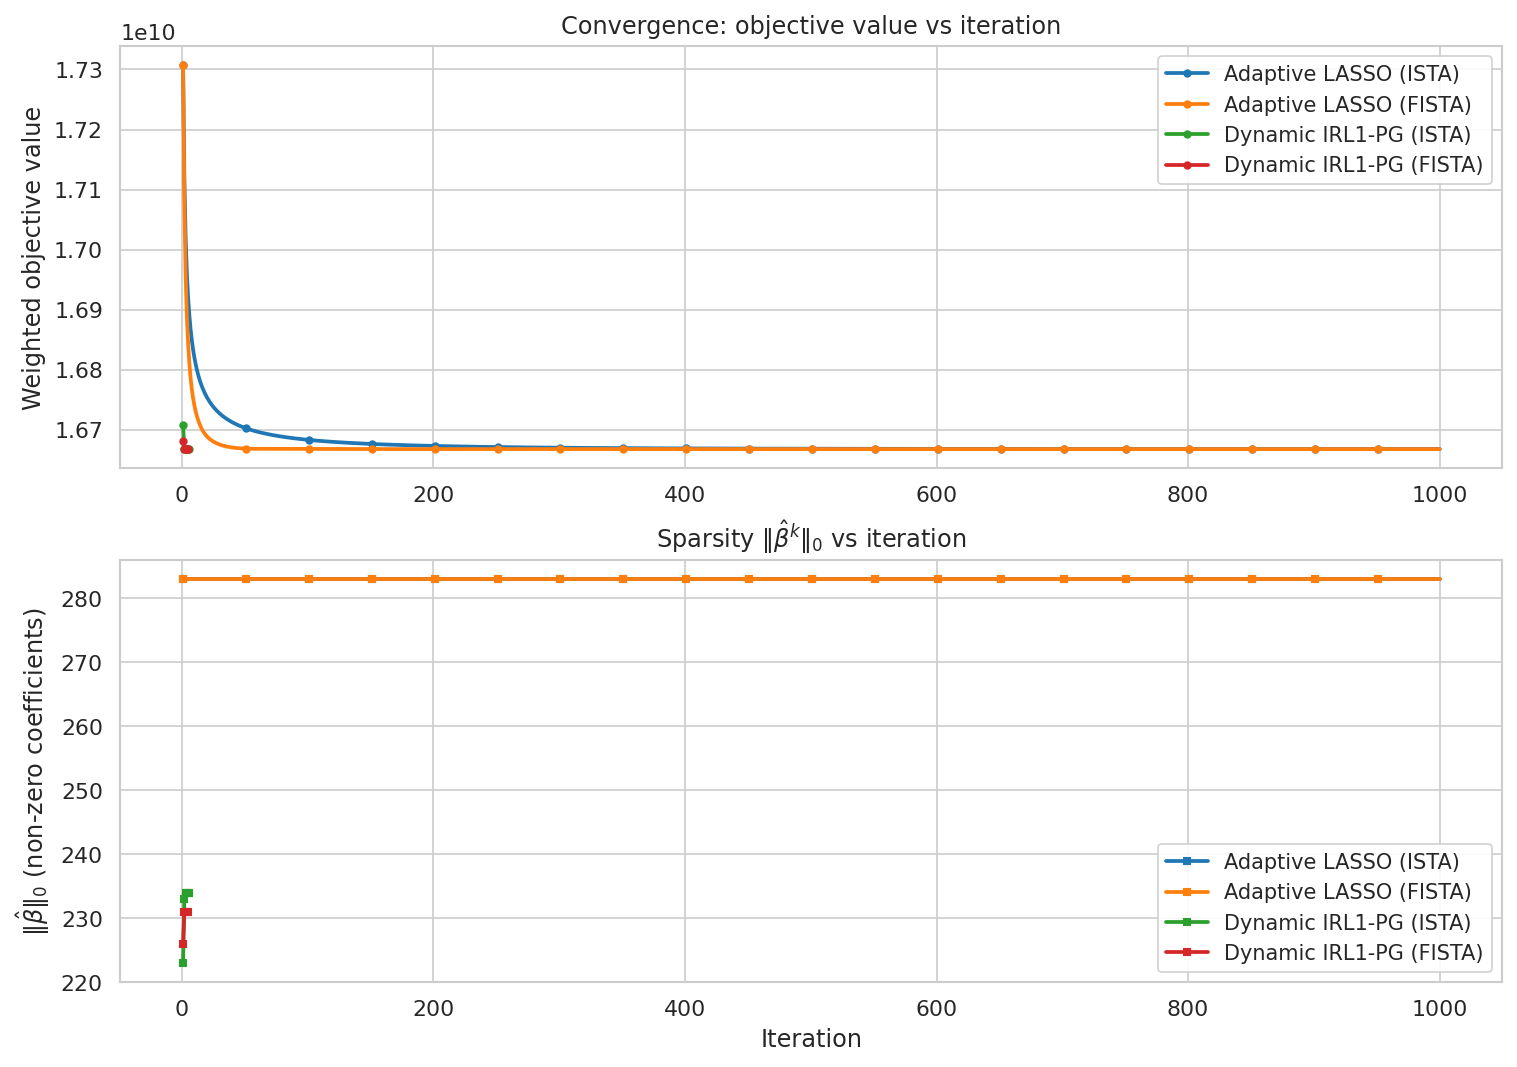
\includegraphics[width=0.95\textwidth]{t16_convergence.png}
    \caption{Convergence plot: objective value vs.\ inner iteration for ISTA,
             FISTA, dynamic IRL1-ISTA, and dynamic IRL1-FISTA.}
    \label{fig:convergence}
\end{figure}

Both dynamic solvers terminate at 2,500 total inner iterations under the selected
configuration (5 outer iterations), while the static adaptive baseline uses 1,000
iterations.  Runtime remains small in absolute terms (about 0.21 seconds for dynamic
methods), and FISTA and ISTA are nearly identical in wall-clock time for this problem
size.  The convergence traces also show that dynamic variants stabilise at much lower
sparsity levels than the static adaptive baseline.

\subsection{Sparsity--Accuracy Trade-off}

\begin{figure}[H]
    \centering
    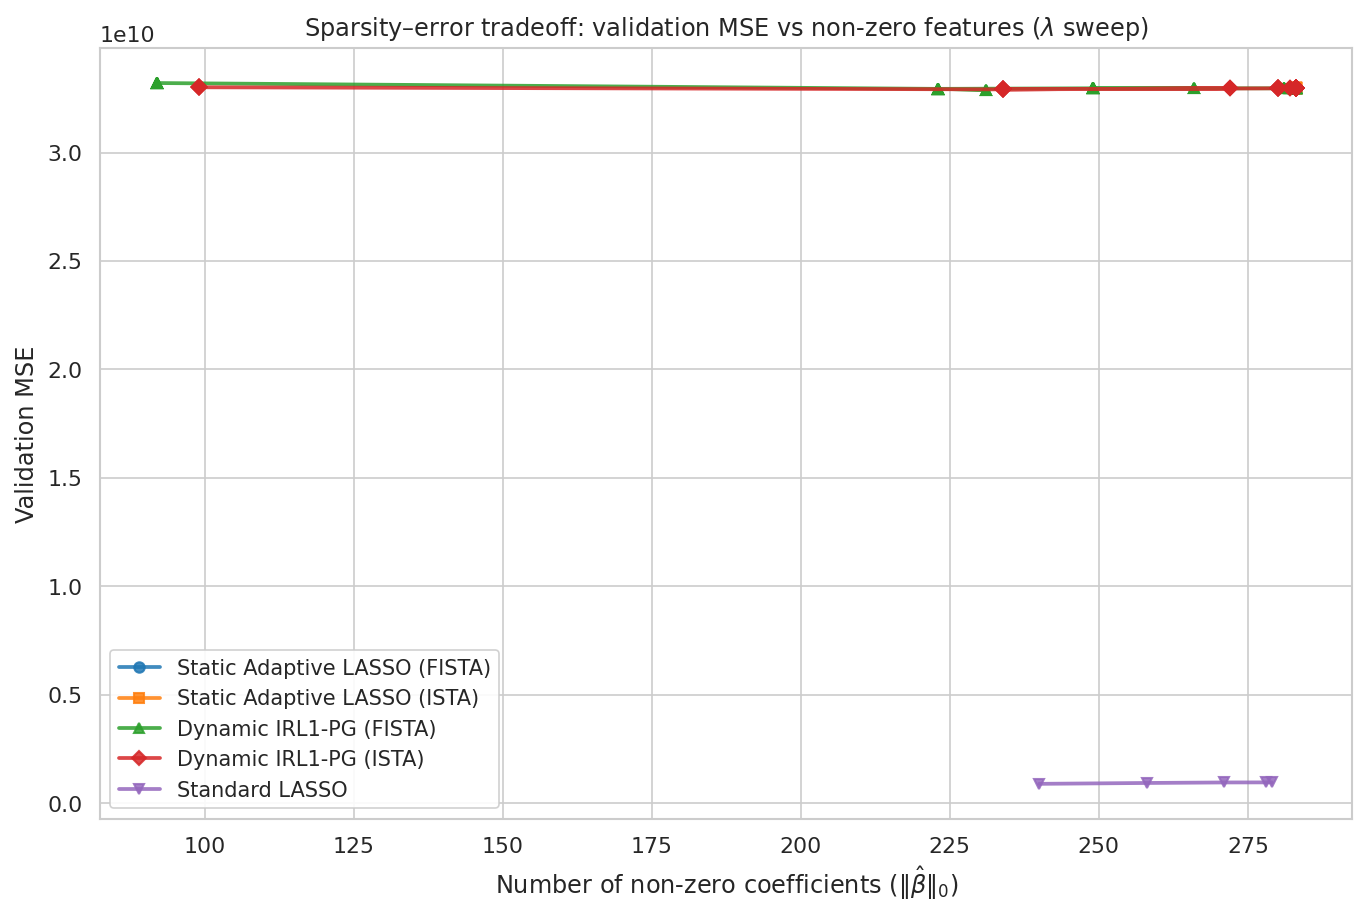
\includegraphics[width=0.95\textwidth]{t17_sparsity_error_tradeoff.png}
    \caption{Validation MSE vs.\ number of non-zero features as $\lambda$ varies.
             Dynamic IRL1-PG variants achieve lower error with substantially fewer
             active coefficients than static adaptive baselines at matched regularisation levels.}
    \label{fig:sparsity}
\end{figure}

The empirical Pareto front confirms that dynamic reweighting can move to lower-$\ell_0$
regions (about 92--99 non-zeros) while maintaining or improving validation error,
compared with the much denser static baselines (about 282--283 non-zeros).

\subsection{Feature Selection Stability}

\begin{table}[H]
\centering
\caption{Feature selection stability loaded from \texttt{stability\_table.csv}.}
\label{tab:stability}
\small
\begin{tabular}{lll}
\toprule
\textbf{Method} & \textbf{Mean Jaccard} & \textbf{Std Jaccard}\\
\midrule
Adaptive LASSO & \fmtjac{0.9872590676518671} & \fmtjac{0.004247102980061563}\\
Dynamic IRL1-FISTA & \fmtjac{0.27212512052234733} & \fmtjac{0.06365032019481207}\\
Dynamic IRL1-ISTA & \fmtjac{0.29228725039449693} & \fmtjac{0.06936056701059536}\\
LASSO & \fmtjac{0.7689303986240856} & \fmtjac{0.018696599399045923}\\
Ridge & \fmtjac{0.9957572112372504} & \fmtjac{0.002643615727941471}\\
\bottomrule
\end{tabular}
\end{table}

The stability profile shows a trade-off: dynamic IRL1-PG improves sparsity and test
error but yields lower support overlap across seeds than static adaptive LASSO.  This
is consistent with stronger pruning near correlated or borderline predictors, where small
data perturbations can change whether a feature survives later reweighting cycles.

\subsection{Feature Interpretation}

Using the best dynamic FISTA run (92 non-zero coefficients), the top absolute
coefficients are dominated by interpretable housing factors from
\texttt{t20\_feature\_interpretation.csv}.  The largest positive effect
is \texttt{GrLivArea} ($+29{,}348$), while large-magnitude negative effects include
\texttt{RoofMatl\_ClyTile} ($-21{,}053$) and \texttt{Condition2\_PosN} ($-9{,}517$).
Strong positive signals also include quality and neighborhood indicators such as
\texttt{GarageQual\_Ex}, \texttt{YearBuilt}, \texttt{OverallQual},
\texttt{Neighborhood\_NoRidge}, and \texttt{Neighborhood\_StoneBr}.  This aligns with
domain expectations: size, build quality, and location remain the strongest
determinants of sale price in the selected sparse model.

\begin{table}[H]
\centering
\caption{Top 10 feature effects loaded from \texttt{t20\_feature\_interpretation.csv}.}
\label{tab:feature-interpretation}
\small
\begin{tabular}{lllp{0.45\textwidth}}
\toprule
\textbf{Feature} & \textbf{Coefficient} & \textbf{Direction} & \textbf{Interpretation}\\
\midrule
\nolinkurl{GrLivArea} & \fmtpred{29348.335138492323} & positive & Size-related feature: larger usable space generally increases price.\\
\nolinkurl{RoofMatl_ClyTile} & \fmtpred{-21052.55427231648} & negative & General structural/categorical feature that appears to decreases price.\\
\nolinkurl{Condition2_PosN} & \fmtpred{-9516.546793622965} & negative & Quality/condition proxy: better values typically decreases price.\\
\nolinkurl{GarageQual_Ex} & \fmtpred{9370.23493013163} & positive & Quality/condition proxy: better values typically increases price.\\
\nolinkurl{YearBuilt} & \fmtpred{8778.704864139238} & positive & Age/renovation signal: newer or renovated homes usually increases price.\\
\nolinkurl{BsmtQual_Ex} & \fmtpred{8553.764965365015} & positive & Quality/condition proxy: better values typically increases price.\\
\nolinkurl{OverallQual} & \fmtpred{8356.406808781141} & positive & Quality/condition proxy: better values typically increases price.\\
\nolinkurl{PoolArea} & \fmtpred{7508.558553473916} & positive & Size-related feature: larger usable space generally increases price.\\
\nolinkurl{GarageCond_Ex} & \fmtpred{-7325.706256396033} & negative & Quality/condition proxy: better values typically decreases price.\\
\nolinkurl{BsmtFinSF1} & \fmtpred{6571.54042063932} & positive & Size-related feature: larger usable space generally increases price.\\
\bottomrule
\end{tabular}
\end{table}

% ══════════════════════════════════════════════════════════════════════════════
\section{Limitations}
\label{sec:limitations}

\begin{enumerate}
    \item \textbf{No global convergence theorem for the outer loop.}
          The ISTA/FISTA convergence rates \citep{beck2009} apply to the inner
          fixed-weight sub-problems.  The outer IRL1 loop changes the objective each
          iteration, so standard convergence bounds do not apply globally.
            We therefore report outer-loop convergence empirically rather than claiming a
            full global proof.

    \item \textbf{No oracle property claim for the dynamic variant.}
          The static Adaptive LASSO has oracle properties under conditions specified by
          \citet{zou2006} and extended by \citet{huang2008}.  The dynamic IRL1 variant
          does not inherit these guarantees automatically; extending oracle property
            analysis to iterative reweighting remains open theoretical work.

    \item \textbf{Efficiency claims are solver-relative.}
          Comparisons of runtime and iteration counts are meaningful only between custom
          ISTA/FISTA variants under matched stopping criteria.  No claim is made that the
          custom implementation outperforms scikit-learn's production coordinate descent.

    \item \textbf{Sensitivity to preprocessing.}
            Results depend on choices in imputation, encoding, and scaling.
          Different preprocessing choices may alter which features are selected and how
          stable that selection is.

    \item \textbf{Single dataset.}
          All empirical conclusions are specific to the House Prices dataset.
          Generalisation to other high-dimensional tabular regression tasks requires
          further evaluation, particularly in the $p \gg n$ regime studied by
          \citet{huang2008}.
\end{enumerate}

% ══════════════════════════════════════════════════════════════════════════════
\section{Conclusion}
\label{sec:conclusion}

We implemented and empirically evaluated IRL1-PG---the Iteratively Reweighted
$\ell_1$ Minimisation framework of \citet{candes2008} integrated with ISTA and FISTA
proximal gradient solvers \citep{beck2009}---for sparse feature selection in
high-dimensional tabular regression.  We applied the method to the House Prices
dataset, where strong feature correlations motivate dynamic reweighting over static
$\ell_1$ penalties \citep{zouhastie2005}.  The IRL1 outer loop sits within the broader
class of reweighted sparsity methods unified by \citet{wipf2011}, while FISTA
acceleration follows Nesterov's \citeyearpar{nesterov1983} momentum framework.

The key findings are: (1) dynamic IRL1-PG produces substantially sparser models
(92--99 non-zeros) than Ridge, LASSO, and static Adaptive LASSO (240--283 non-zeros)
while improving test error on this dataset split; (2) within dynamic variants, ISTA
achieves the best validation MSE while FISTA achieves the best test MSE and MAE with
comparable runtime; and (3) dynamic reweighting improves sparsity--error trade-offs but
reduces support stability across random seeds relative to static adaptive weighting.
We also note practical limits: no global outer-loop convergence theorem is claimed, and
results remain sensitive to preprocessing choices.

Future directions include extending IRL1-PG to generalised linear models, combining it
with group-sparse penalties for handling structured correlations \citep{zouhastie2005},
and applying it to higher-dimensional genomics or financial datasets where the $p \gg n$
regime is more extreme \citep{huang2008}.

% ══════════════════════════════════════════════════════════════════════════════
\bibliographystyle{plainnat}
\begin{thebibliography}{99}

\bibitem[Beck and Teboulle(2009)]{beck2009}
Beck, A.\ and Teboulle, M.\ (2009).
\newblock A fast iterative shrinkage-thresholding algorithm for linear inverse
  problems.
\newblock \emph{SIAM Journal on Imaging Sciences}, 2(1):183--202.
\newblock \doi{10.1137/080716542}.

\bibitem[Cand{\`e}s et al.(2008)]{candes2008}
Cand{\`e}s, E.~J., Wakin, M.~B., and Boyd, S.~P.\ (2008).
\newblock Enhancing sparsity by reweighted $\ell_1$ minimization.
\newblock \emph{Journal of Fourier Analysis and Applications},
  14(5--6):877--905.
\newblock \doi{10.1007/s00041-008-9045-x}.

\bibitem[Daubechies et al.(2009)]{daubechies2009}
Daubechies, I., DeVore, R., Fornasier, M., and G{\"u}nt{\"u}rk, C.~S.\ (2009).
\newblock Iteratively reweighted least squares minimization for sparse
  recovery.
\newblock \emph{Communications on Pure and Applied Mathematics},
  63(1):1--38.
\newblock \doi{10.1002/cpa.20303}.

\bibitem[Huang et al.(2008)]{huang2008}
Huang, J., Ma, S., and Zhang, C.-H.\ (2008).
\newblock Adaptive {Lasso} for sparse high-dimensional regression models.
\newblock \emph{Statistica Sinica}, 18(4):1603--1618.

\bibitem[Kaggle(2019)]{kaggle2019}
Kaggle (2019).
\newblock House {Prices}: {Advanced} {Regression} {Techniques}.
\newblock \url{https://www.kaggle.com/competitions/house-prices-advanced-regression-techniques}.

\bibitem[Nesterov(1983)]{nesterov1983}
Nesterov, Y.~E.\ (1983).
\newblock A method for solving the convex programming problem with convergence
  rate $O(1/k^2)$.
\newblock \emph{Doklady Akademii Nauk SSSR}, 269(3):543--547.

\bibitem[Parikh and Boyd(2014)]{parikh2014}
Parikh, N.\ and Boyd, S.\ (2014).
\newblock Proximal algorithms.
\newblock \emph{Foundations and Trends in Optimization}, 1(3):127--239.
\newblock \doi{10.1561/2400000003}.

\bibitem[Tibshirani(1996)]{tibshirani1996}
Tibshirani, R.\ (1996).
\newblock Regression shrinkage and selection via the lasso.
\newblock \emph{Journal of the Royal Statistical Society, Series B},
  58(1):267--288.

\bibitem[Wipf and Nagarajan(2011)]{wipf2011}
Wipf, D.\ and Nagarajan, S.\ (2010).
\newblock Iterative reweighted $\ell_1$ and $\ell_2$ methods for finding sparse
  solutions.
\newblock \emph{IEEE Journal of Selected Topics in Signal Processing},
  4(2):317--329.
\newblock \doi{10.1109/JSTSP.2010.2042413}.

\bibitem[Zou(2006)]{zou2006}
Zou, H.\ (2006).
\newblock The adaptive lasso and its oracle properties.
\newblock \emph{Journal of the American Statistical Association},
  101(476):1418--1429.
\newblock \doi{10.1198/016214506000000735}.

\bibitem[Zou and Hastie(2005)]{zouhastie2005}
Zou, H.\ and Hastie, T.\ (2005).
\newblock Regularization and variable selection via the elastic net.
\newblock \emph{Journal of the Royal Statistical Society, Series B},
  67(2):301--320.
\newblock \doi{10.1111/j.1467-9868.2005.00503.x}.

\end{thebibliography}

\end{document}
